\documentclass{article}

\usepackage{booktabs}
\usepackage{multirow}
\usepackage{amsmath}
\usepackage{hyperref}
\usepackage{overpic}
\usepackage{amssymb}
\usepackage{graphicx}
\usepackage{tikz}
\usepackage{pgf-pie}

\usepackage[accepted]{dlai2025}

\dlaititlerunning{Audio Super-Resolution using Deep Learning - }

\begin{document}

\twocolumn[
\dlaititle{Audio Super-Resolution using Deep Learning}

\begin{center}\today\end{center}

\begin{dlaiauthorlist}
    \dlaiauthor{Kevin Cukaj}{1}
    \dlaiauthor{Cesare Corsi}{1}
\end{dlaiauthorlist}

\dlaiaffiliation{1}{University of Sapienza}

\dlaicorrespondingauthor{Kevin Cukaj}{cukaj.1942958@studenti.uniroma1.it}
\dlaicorrespondingauthor{Cesare Corsi}{corsi.2156214@studenti.uniroma1.it}


\vskip 0.3in
]

\printAffiliationsAndNotice

\begin{abstract}
This paper presents a deep learning approach for audio super-resolution.
We implement a U-Net architecture with skip connections that directly operates on raw waveforms.
Our method captures both temporal and frequency characteristics of audio signals, effectively reconstructing the high-frequency components lost in low-resolution recordings.
Experimental results demonstrate improvements in both objective metrics and subjective quality when applied to music samples from the Free Music Archive (FMA) dataset.
\end{abstract}

% ------------------------------------------------------------------------------
\section{Introduction}

Audio super-resolution refers to the process of reconstructing high-resolution audio signals from their low-resolution counterparts. 
This task is particularly challenging because audio signals contain complex temporal and spectral features that are easily lost when downsampled to lower rates.
Current approaches often rely on signal processing techniques that have limitations in recovering the fine details of audio signals.

In this project, we address the problem of increasing the sampling rate of audio from 16 kHz to 44.1 kHz, effectively recovering the high-frequency components (above 8 kHz) that are lost in the downsampling process.
We propose a deep learning approach based on a modified U-Net architecture that operates directly on raw waveforms rather than time-frequency representations, allowing end-to-end training and inference without intermediate transformations.

The code for this project is available at: \url{https://github.com/KevinCukaj/deep-learning-project}.

% ------------------------------------------------------------------------------
\section{Related Work}

Multiple models such as AudioSR \cite{liu2024audiosr} and NU-Wave2 \cite{han2022nu} were tested.
These two models were first considered as a starting point for our project.
Unfortunately, they were not suitable for our task because either the checkpoint was not available or dependencies conflicts that we could not resolve.
Also, the AudioSR model performances' were not satisfactory in the Colab environment, in which we would not even get an output because of the memory limitations.

% ------------------------------------------------------------------------------
\section{Method}

\subsection{Problem Formulation}
Let $x_{\text{LR}} \in \mathbb{R}^n$ be a low-resolution audio signal sampled at 16 kHz, and $x_{\text{HR}} \in \mathbb{R}^m$ be the corresponding high-resolution signal at 44.1 kHz, where $m > n$. Our goal is to learn a mapping function $f_\theta: \mathbb{R}^n \rightarrow \mathbb{R}^m$ such that $f_\theta(x_{\text{LR}}) \approx x_{\text{HR}}$.

\subsection{Dataset Preparation}
We create paired training examples using the Free Music Archive (FMA) dataset \cite{fma_dataset}. 
For each high-resolution audio clip $x_{\text{HR}}$, we generate its low-resolution counterpart $x_{\text{LR}}$ through the following process:
\begin{enumerate}
    \item Downsample $x_{\text{HR}}$ from 44.1 kHz to 16 kHz,
    \item Upsample back to 44.1 kHz using basic interpolation,
    \item Apply a low-pass filter with cutoff at 60\% of the Nyquist frequency (4.8 kHz). The 60\% value represents a good balance between preserving enough information for the model to learn meaningful correlations.
\end{enumerate}

This procedure simulates the bandwidth limitation of low-sampling rate audio while ensuring both signals have the same dimensions for training.

\subsection{Network Architecture}
We implement a modified U-Net architecture with four encoding and decoding blocks.
The encoder path consists of 1D convolutional layers followed by batch normalization and LeakyReLU activations.
The decoder path uses transposed convolutions with ReLU activations and also includes batch normalization.

Skip connections link the encoder and decoder at corresponding levels, helping preserve fine details that might otherwise be lost in the bottleneck.
The network takes as input a segment of low-resolution audio and outputs the corresponding high-resolution audio of the same length.

The model can be formalized as:
\begin{equation}
\hat{x}_{\text{HR}} = f_\theta(x_{\text{LR}})
\end{equation}

\subsection{Training Procedure}
As a first attempt, we used the L1-loss as our primary loss function.
Although this still produced a decent reconstruction, L1 and L2 don't reflect natural biases in human hearing since we perceive certain frequencies to be louder or quieter than others.
This is why we decided to use a perceptual loss function like STFT (Short-Time Fourier Transform) loss, which captures the frequency content of the audio signal more effectively.
The STFT loss is computed as follows:
\begin{equation}
\mathcal{L}_{\text{STFT}}(\theta) = ||\text{STFT}(f_\theta(x_{\text{LR}})) - \text{STFT}(x_{\text{HR}})||_1
\end{equation}

% ------------------------------------------------------------------------------
\section{Experimental Results}

\subsection{Implementation Details}
The model was trained on the FMA small dataset containing approximately 8,000 tracks of 30-second audio clips across various genres.
Since the computational power at our disposal was very limited, and Google Colab's free plan has its limitations, we ended up using a subset of just 2000 tracks for training.

We used an 80/10/10 split for training, validation, and testing. Training was performed on a single GPU with a batch size of 16 for 100 epochs.

The segment length (fixed-duration chunk or slice of an audio signal that is extracted and used as an input unit for a model) was set to 16384 samples (approximately 372 ms at 44.1 kHz).
This was done to cope with the memory limitations of the Colab environment.

We added support for resuming training from previously saved checkpoints, allowing us to bypass Colab's session time limits and continue training seamlessly across multiple days.
Of course, the original dataset split used at the start of training was preserved for consistency reasons.

\subsection{Hyperparameter Tuning}
To find good hyperparameter values, several training runs were performed.
The final values were chosen based on the best validation loss achieved during training.  

The learning rate was initialized at 0.001, and we used the Adam optimizer with a ReduceLROnPlateau scheduler that reduces the learning rate by a factor of 0.5 when validation loss does not improve for 5 epochs.

\subsection{Evaluation Metrics}
We evaluate our model using both objective metrics and subjective evaluation:
\begin{itemize}
    \item L1 Loss: Measures the absolute difference between predicted and ground truth samples
    \item MSE Loss: Measures the squared error between predicted and ground truth samples
    \item STFT Loss: Measures the difference in frequency content between predicted and ground truth audio
    \item Qualitative assessment: human listeners evaluate the perceptual quality of the enhanced audio comparing it to the low-resolution counterpart.
\end{itemize}

\subsection{Results and Discussion}
Our model can reconstruct high-frequency components lost in low-resolution audio. 
The training process is illustrated in Figure \ref{fig:training}, with respect to the STFT loss.

\begin{figure}[!htb]
    \centering
    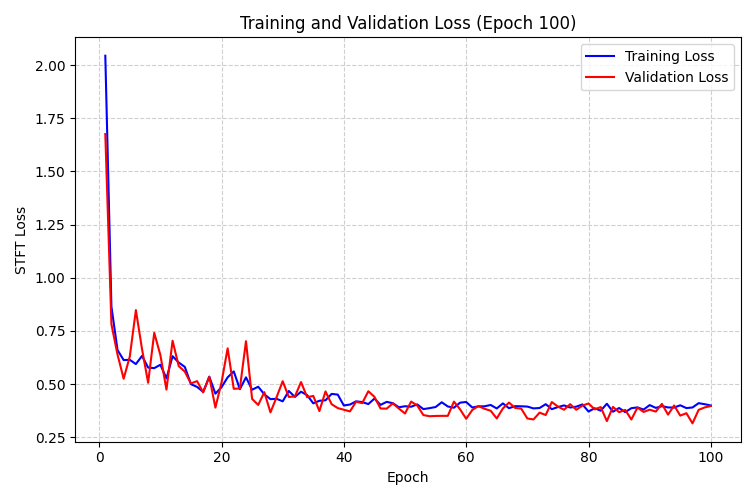
\includegraphics[width=1\linewidth]{images/training.png}
    \vspace{-0.7cm} % Reduce space between image and caption
    \caption{Training and validation losses over epochs}
    \label{fig:training}
\end{figure}

Quantitatively, we achieve the losses presented on Table \ref{tab:results} on the test set.

\begin{table}[!htb]
    \centering
    \begin{tabular}{lc}
        \toprule
        \textbf{Metric} & \textbf{Value} \\
        \midrule
        Average L1 Loss & 0.4785 \\
        Average MSE Loss & 0.3805 \\
        Average STFT Loss & 0.3366 \\
        \bottomrule
    \end{tabular}
    \caption{Quantitative results of audio super-resolution}
    \label{tab:results}
\end{table}

As a subjective evaluation method, MOS (Mean Opinion Score) was used, where the low and high versions of the same audio sample were given to 20 listeners.
Each had to give a score from 1 (Bad) to 5 (Excellent) based on their listening experience.
The pie chart in Figure \ref{fig:qualitative} summarizes the listeners' feedback on the restored sample.

\begin{figure}[!htb]
    \centering
    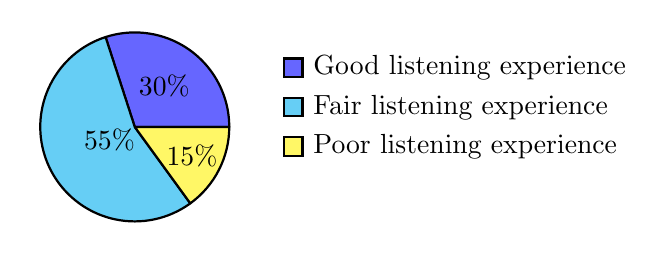
\begin{tikzpicture}
        \pie[
            radius=1.2,
            text=legend,
            after number={\%},
        ]{30/Good listening experience, 55/Fair listening experience, 15/Poor listening experience}
    \end{tikzpicture}
    \caption{Subjective evaluation of restored audio sample}
    \label{fig:qualitative}
\end{figure}

The final MOS score was
\begin{align*}
    \text{MOS} &= \frac{(5 \cdot 0) + (4 \cdot 6) + (3 \cdot 11) + (2 \cdot 3) + (1 \cdot 0)}{20} \\
    &= 3.15
\end{align*}

All of the listeres reported that the restored audio sample sounded more detailed compared to the low-resolution version.

% ------------------------------------------------------------------------------
\section{Conclusion and Future Work}

We presented a deep learning approach for audio super-resolution that is able to reconstruct high-frequency components from low-resolution audio, through a U-Net architecture that operates directly on raw waveforms.

One could possibly achieve better results by using a larger and more diverse dataset, as well as experimenting more with different combinations of hyperparameters.
Also, a longer trainging time could provide better results, as the model was trained for only 100 epochs due to computational constraints.

The primary limitation of our current approach is the segment-by-segment processing, which could introduce discontinuities at segment boundaries.
Implementing overlap-add techniques or recurrent components could address this limitation in future iterations.

\bibliography{references}
\bibliographystyle{dlai2025}

\end{document}